\begin{figure}
	
  \setlength{\unitlength}{\textwidth}

\fbox{
        \begin{picture}(1,1.3)(0,0.5)

      % % % Parkinson Data 

      \put(0.05,0.52){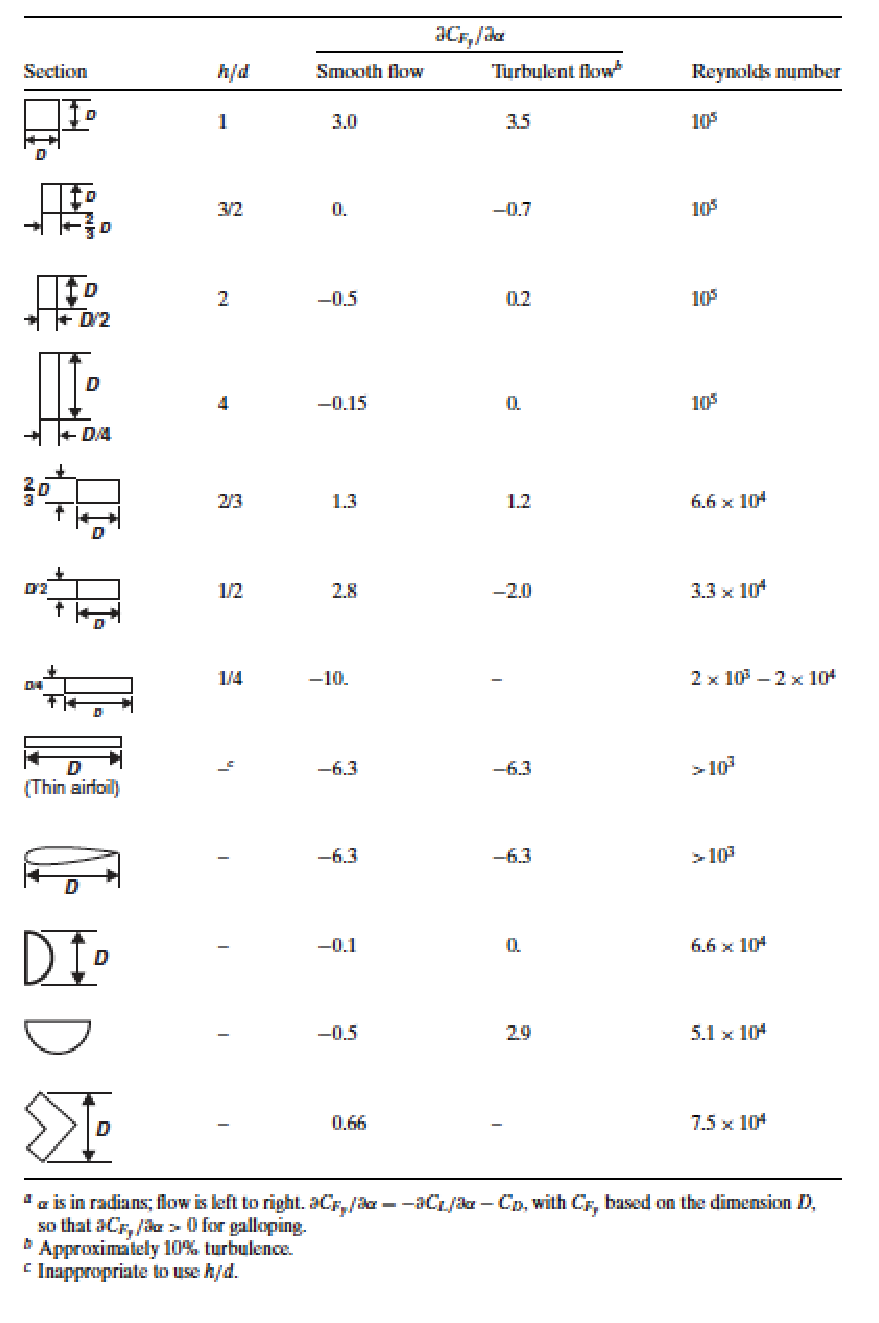
\includegraphics[width=0.8\unitlength]{./chapter-literature-revirw/fnp/per_cross_sec.eps}}
        


    \end{picture}
}
  \caption{ ``The transverse force coefficient for various sections in steady smooth or turbulent flow (after \citet{Blevins1990})" obtained from \citet{Paidoussis2010}}
    \label{fig:par_diff_cross_sec}
\end{figure}

 %vspace{10cm}
